\chapter{Diskussion}
\label{chap:diskussion}
\section{Interpretation der Ergebnisse}
\todo{Hier nochmal den Inhalt überdenken.}
Erfolg der Implementierung:
Was hat gut funktioniert? Wo gab es unerwartete Herausforderungen?

Einsatz in der Praxis:
Inwiefern ist das Ergebnis in der Praxis anwendbar? Welche Verbesserungen sind nötig?

Vergleich mit bestehenden Lösungen:
Falls bekannt, könnten Sie Ihre Lösung mit anderen Ansätzen vergleichen.

\section{Limitation}
\label{sec:limitationen}
Die Analyse und Implementierung unterliegt spezifischen Einschränkungen, die sowohl durch methodische als auch durch technologische Faktoren bedingt sind. Dabei sind insbesondere die Generalisierbarkeit der Ergebnisse und die Abdeckung aller relevanten Daten kritisch zu betrachten. \todo{Über "Generalisierbarkeit der Ergebnisse und die Abdeckung aller relevanten Daten" noch schreiben oder hier streichen.} Weiterhin beeinflussen die Auswahl und die Qualität der genutzten Datenquellen sowie deren Aktualität die Aussagekraft der Analyse. \todo{Diesen Absatz nochmal betrachten.}
\subsection{Generelle Limitationen}
\label{limitation-generell}
\par Die \gls{nvd} gilt als zentrale Resource für Informationen über öffentlich bekannte Sicherheitslücken. Daher scheint es auch als verlässliche Quelle für die IT-Sicherheitsbranche und Forschungszwecke. Laut einer Veröffentlichung vom 13. Februar 2024 kommt das \gls{nist} nicht der Abarbeitung der eingereichten \glspl{cve} hinterher und arbeitet daran, die Verzögerung bei der Analyse zu beheben \autocite{NVDProgramAnnouncement}. Am 13. November 2024 kündigte das \gls{nist} an, alle neu eingereichten \gls{cve} direkt verarbeiten zu können. Die Abarbeitung der zurückgestellten Daten dauert weiterhin an. Die Daten aus der \gls{nvd} sind daher aktuell  nicht auf dem neusten Stand \autocite{NationalVulnerabilityDatabase2024}. Eine vom \textit{IT Security Infrastructures Lab} der \textit{Friedrich-Alexander Universität Erlangen-Nürnberg} veröffentliche Studie vom \citedate{wunderNVDUsersAttitudes2024} unterlegt diese Feststellung mit empirischen Daten. Demnach sind fast 40\% der Befragten jährlich, monatlich, wöchentlich oder täglich von der verzögerten Veröffentlichung von neuen \glspl{cve} betroffen \autocite{wunderNVDUsersAttitudes2024}. Die damit zusammenhängenden und weitere technische Schwierigkeiten beeinflussen auch die Abfrageverfügbarkeit und Abfragegeschwindigkeit von Daten aus der \gls{nvd}. Für \gls{acema} haben die Einschränkungen weitreichende Konsequenzen, von verlangsamter Abfragegeschwindigkeit des \gls{cvss} für \glspl{cve} bis hin zur vollständigen Abwesenheit von \gls{cvss} Daten, die eine integrale Rolle für die Datenanalyse spielen.
%
\subsection{Limitation von ACEMA}
\label{limitationen-acema}
Die Implementierung von \gls{acema} nutzt für die Bewertung das \gls{cvss} in Version \textit{v2.0} aus dem Jahr 2007 \autocite{Acema_oranOCloud_Data_GatheringpyMaster}. Seit dem 27. Juni 2024 unterstützt die \gls{nvd} das Bereitstellen von Daten in \textit{v4.0} des \gls{cvss} \autocite{NVDCVSSV40}. Nicht nur ist die in \gls{acema} genutzte Version durch zwei \textit{major}-Versionen überholt, seit dem 13. Juli 2022 werden in der Datenbank keine neuen Angriffsvektordaten, qualitative Schweregrad-Bewertungen oder Schweregrad-Werte in \gls{cvss} \textit{v2.0} erstellt \autocite{RetirementCVSSV2}. Der Fall von unvollständigen Daten ist in der Bearbeitung dieses Projekts nicht vorgekommen, da alle im Ergebnisse des Mappings aufgeführten \glspl{cve} im Jahr 2021 oder früher veröffentlicht wurden. Es ist jedoch theoretisch möglich, dass diese Einschränkung bei der weiteren Nutzung dieser Methode zu fehlenden Daten führen kann.
%
\par Das von \gls{acema}, mithilfe des \gls{cti} Repositories, erstellte Mapping von \gls{mitre}-Technik zu \gls{capec} (Schritt 1 in Abbildung \ref{fig:mitre_mapping}) findet nicht alle \gls{capec}. Die Dokumentation im Repository erklärt zu dem Finden von \glspl{capec}: \gls{capec} IDs können dort für die Techniken gefunden werden, wo das unter externen Referenzen das Attribut \textit{source\_name} den Wert \verb|capec| hat \autocite{CtiUSAGEmdMaster} \autocite{CtiUSAGECAPECmdMaster}. \citeauthor{klementSecuring6GTransition2024} nutzen in ihrer Implementierung die Daten aus dem \textit{enterprise-attack/attack-pattern} Teil des Repositories \autocite{klement2023acema}. Nach demselben Prinzip kann auch der \textit{capec/2.1/attack-pattern} Teil des Repositories durchsucht werden. Der Unterschied in den beiden Datensätzen liegt darin, was der Hauptzweck der Daten ist. Der \textit{enterprise-attack} Teil enthält die Datenstruktur \todo{anderes Wort für Datenstruktur} der \gls{mitre} \gls{attack} \textit{Enterprise}-Matrix, mit Daten wie der \gls{mitre}-Technik ID, Taktik und angreifbare Platform sowie manchmal Referenzen zu \gls{mitre}-Techniken. Der \gls{capec} Teil enthält die Datenstruktur \todo{anderes Wort für Datenstruktur} des \gls{capec}-Frameworks, mit Daten wie \gls{capec} ID, Konsequenzen und Voraussetzungen für die Ausnutzung sowie manchmal Referenzen zu \gls{mitre}-Techniken. Es zeigt sich in den Daten aus Tabelle \ref{tab:comparison_with_diff}, dass über den \textit{\gls{capec}} Teil eine vollständigere Abbildung von \gls{mitre}-Technik zu \gls{capec} ID möglich ist. Die beiden Implementierungen des Mappings wurden auf demselben Datensatz aus Anhang \ref{app:mapping-dataset} ausgeführt, der ein direkter Export der Daten aus der Dashboardmatrix ist.
%

\begin{table}[H]
    \centering
    \caption{Vergleich der Daten zwischen eigener Implementierung und ACEMA Implementierung inklusive prozentualer Differenzen}
    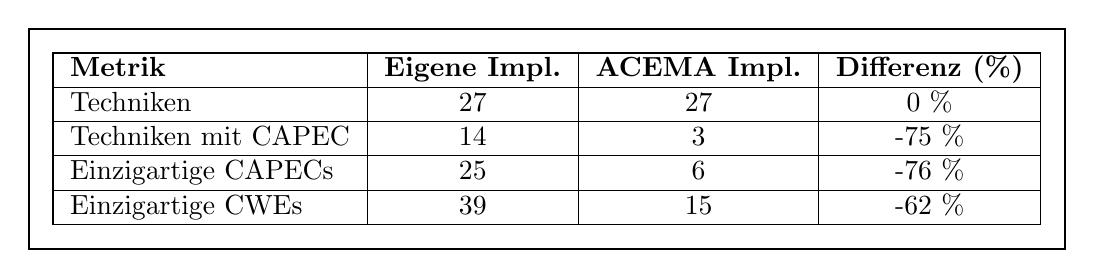
\begin{tikzpicture}
        \node[draw, thick, inner sep=3mm, rectangle] (table) {
        \begin{tabular}{|l|c|c|c|}
        \hline
        \textbf{Metrik} & \textbf{Eigene Impl.} & \textbf{ACEMA Impl.} & \textbf{Differenz (\%)} \\
        \hline
        Techniken & 27 & 27 & 0 \% \\
        \hline
        Techniken mit CAPEC & 14 & 3 & -75 \% \\
        \hline
        Einzigartige CAPECs & 25 & 6 & -76 \% \\
        \hline
        Einzigartige CWEs & 39 & 15 & -62 \% \\
        \hline
        \end{tabular}
    };
    \end{tikzpicture}
\label{tab:comparison_with_diff}
\end{table}

\section{Ausblick}
\label{sec:ausblick}
Starten von \gls{acema} aus dem Dashboard heraus, dafür entweder \gls{acema} in GoLang implementieren oder python Wrapper oä\dots \\
Live-Updates im Dashboard, wenn neue Artefakte eingefügt oder Kampagnen starten. \\
Mapping von Technik zu CVE auch für MS-Techniken implementieren. \\
Aus \gls{acema}: Manuelle Zuordnung unterstützen durch maschinelles Lernen. \\

